% =====================================================================
%  Chương 3 (tiếp) — Kết quả thực nghiệm và phân tích an toàn mở rộng
% =====================================================================

\section{Kết quả thực nghiệm}
\label{sec:ketqua}

\subsection{Dữ liệu, môi trường và kịch bản thực nghiệm}

Ảnh phủ là toàn bộ 8000 ảnh của bộ dữ liệu Linnaeus 5 \cite{chaladze2017}, gồm 5 lớp
(\hinh{fig:linnaeus}), mỗi lớp 1200 ảnh huấn luyện và 400 ảnh kiểm tra, kích thước $256\times256$.
Ảnh bí mật là ảnh xám ``coins'', lấy từ \code{skimage.data.coins()} và chuẩn hóa về kích thước
\code{coins.png} của MATLAB ($246\times300$) bằng nội suy \code{INTER\_AREA}. Cấu hình máy chạy thực
nghiệm được nêu ở \bang{tab:env}.

\begin{figure}[H]
\centering
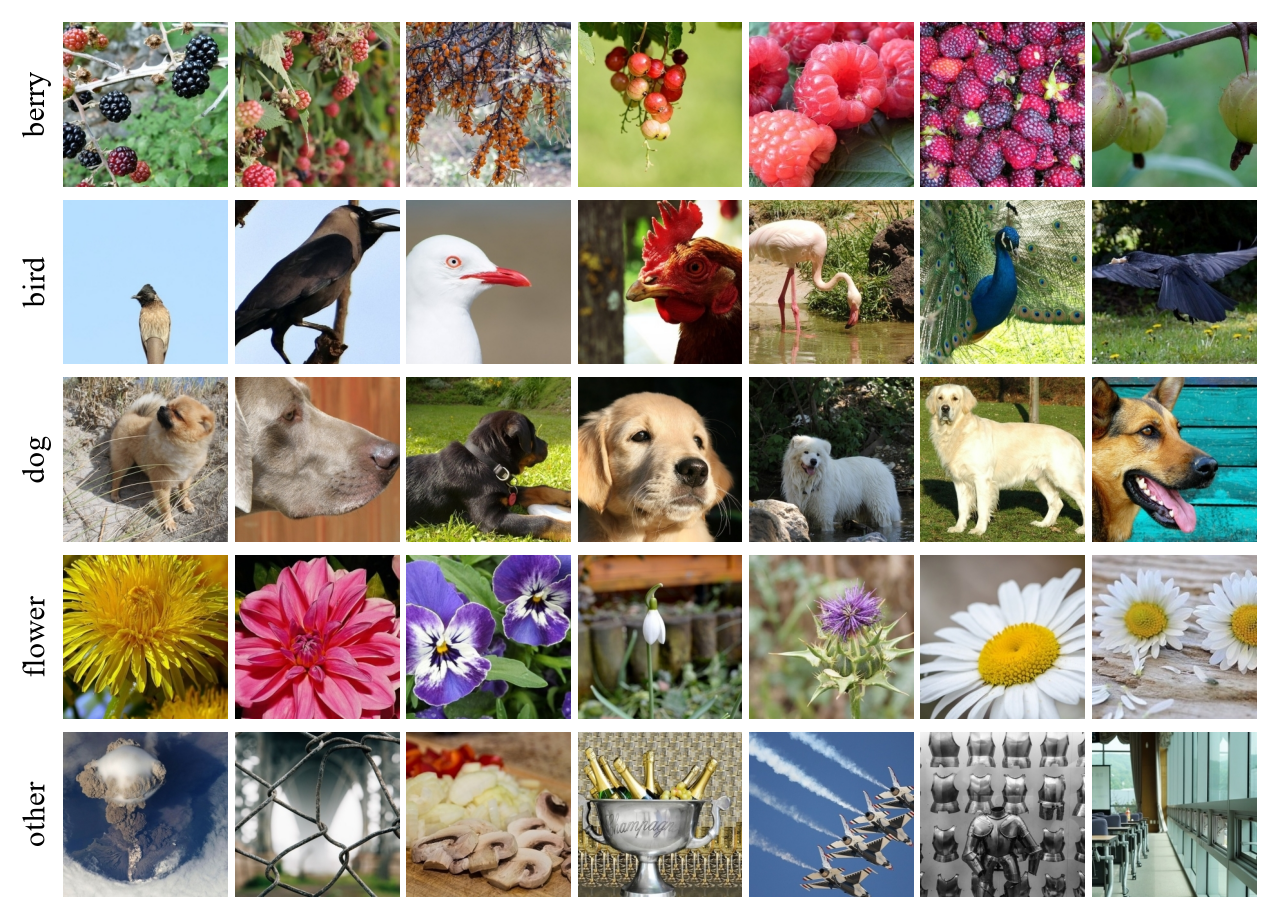
\includegraphics[width=0.86\linewidth]{linnaeus5_samples}
\caption{Một số ảnh phủ của bộ dữ liệu Linnaeus 5 (mỗi hàng là một lớp)}
\label{fig:linnaeus}
\end{figure}

\begin{table}[H]
\centering
\caption{Môi trường thực nghiệm}
\label{tab:env}
\small
\begin{tabularx}{0.85\linewidth}{@{}P{3.6cm}L@{}}
\toprule
\thead{Thành phần} & \thead{Cấu hình}\\
\midrule
Bộ xử lý & Intel Core i3-1005G1 (2 nhân, 4 luồng, xung cơ bản 1.20 GHz, hỗ trợ AES-NI)\\
Bộ nhớ & 20 GB RAM\\
Hệ điều hành & Windows 11 IoT Enterprise LTSC 2024 (64 bit)\\
Phần mềm & Python 3.12.8 và các thư viện ở \bang{tab:tech}\\
\bottomrule
\end{tabularx}
\end{table}

Theo quyết định BM-01, thực nghiệm được tổ chức thành hai kịch bản bổ sung cho nhau
(\bang{tab:scenarios}).

\begin{table}[H]
\centering
\caption{Hai kịch bản thực nghiệm}
\label{tab:scenarios}
\small
\begin{tabularx}{\linewidth}{@{}P{3.2cm}LL@{}}
\toprule
\thead{Thuộc tính} & \thead{Kịch bản A -- một cặp ảnh} & \thead{Kịch bản B -- benchmark}\\
\midrule
Mục đích & Tái hiện Hình~4 và Hình~5 & Tái hiện Bảng~2\\
Ảnh phủ & Ảnh mẫu \code{berry} & 8000 ảnh Linnaeus 5\\
Ảnh bí mật & $246\times300$ (\num{73800} byte) & $156\times156$ (\num{24336} byte)\\
Số bit LSB & 3 (ảnh phủ phóng to lên $257\times257$) & 1 (không phóng to)\\
Số lượt chạy & 3 (một lượt mỗi thuật toán) & \num{24000} ($8000 \times 3$)\\
Chaotic khi đo EncTime & Sinh lại mặt nạ mỗi lần & Cache mặt nạ (\code{--cache-chaotic-mask})\\
Kịch bản dòng lệnh & \code{scripts.run\_single} & \code{scripts.run\_benchmark --secret-size 156 156}\\
\bottomrule
\end{tabularx}
\end{table}

\subsection{Kết quả trên một cặp ảnh mẫu}

\hinh{fig:fig4} và \hinh{fig:fig5} là kết quả tái hiện Hình~4 và Hình~5 của bài báo. Histogram
ảnh phủ và ảnh bí mật (\hinh{fig:fig4}) có hình dạng tương tự bài báo: ảnh phủ có một đỉnh lớn
quanh mức 100--130, còn ảnh ``coins'' tập trung ở vùng tối 30--60 do nền ảnh. Ở \hinh{fig:fig5},
bản mã của cả ba thuật toán trông như nhiễu ngẫu nhiên, histogram phẳng với khoảng 288 điểm ảnh
mỗi mức, và histogram ảnh stego giữ nguyên hình dạng histogram ảnh phủ.

\begin{figure}[H]
\centering
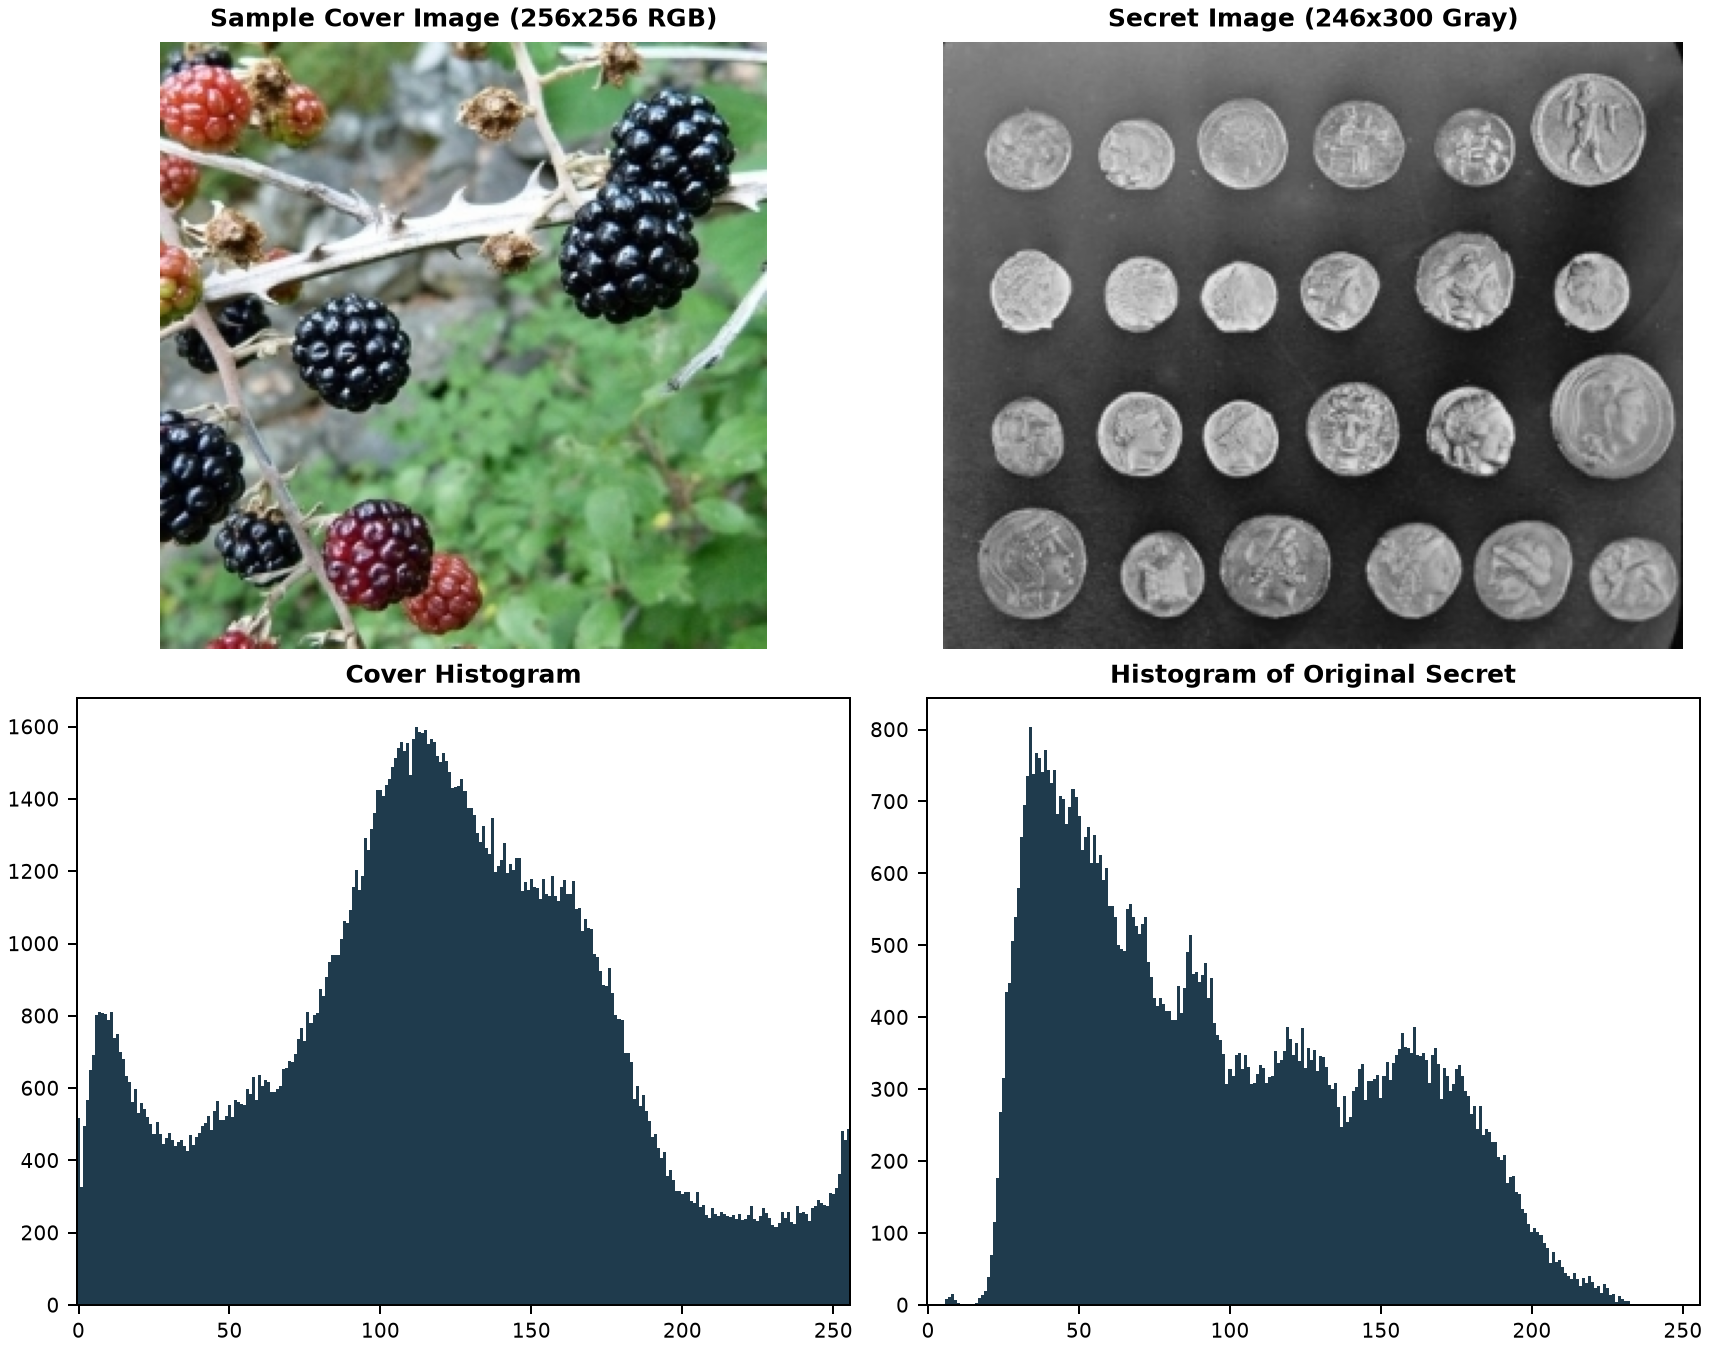
\includegraphics[width=0.82\linewidth]{fig4_cover_secret_histograms}
\caption{Tái hiện Hình~4 của bài báo: ảnh phủ, ảnh bí mật và histogram tương ứng}
\label{fig:fig4}
\end{figure}

\begin{figure}[H]
\centering
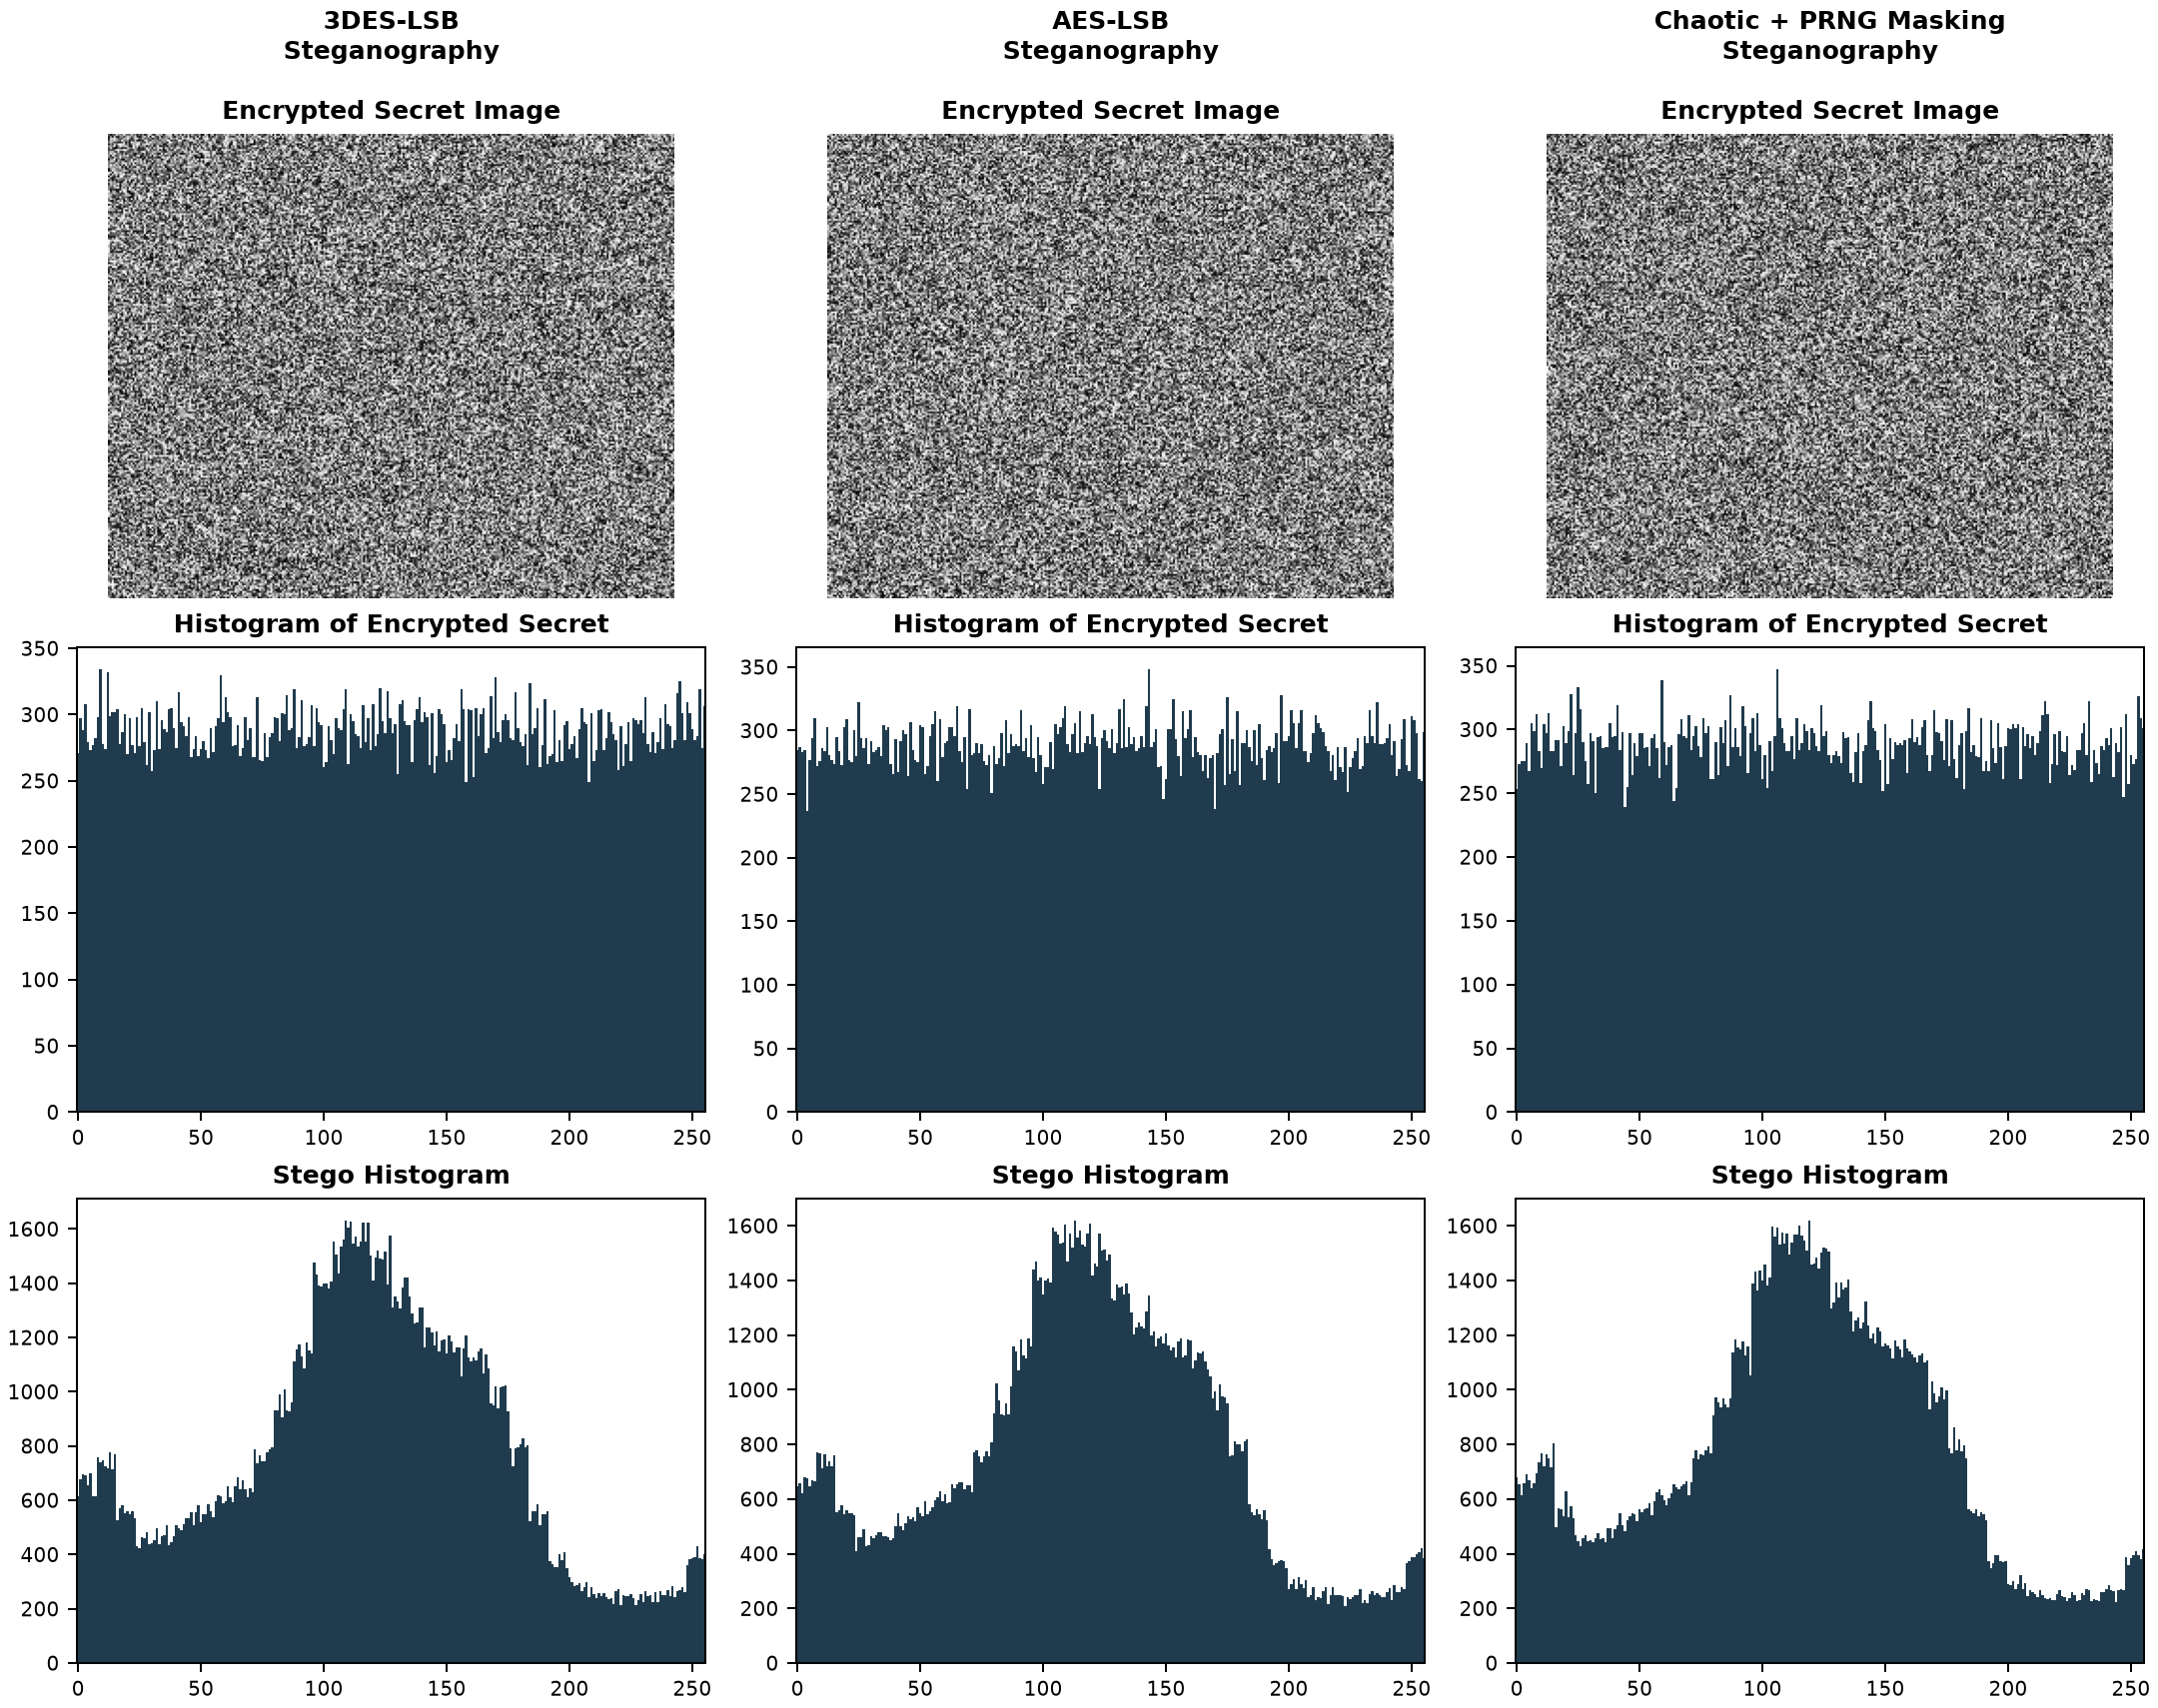
\includegraphics[width=0.92\linewidth]{fig5_comparison_grid}
\caption{Tái hiện Hình~5 của bài báo: bản mã, histogram bản mã và histogram ảnh stego của
3DES-LSB, AES-LSB và Chaotic-LSB (ảnh bí mật $246\times300$)}
\label{fig:fig5}
\end{figure}

\bang{tab:single} trình bày các độ đo của kịch bản A. Cả ba thuật toán đều khôi phục ảnh bí mật
chính xác tuyệt đối. Do tải tin \num{73800} byte vượt dung lượng 3-LSB của ảnh $256\times256$, hệ
thống tự động chọn $k = 3$ và phóng to ảnh phủ lên $257\times257$. MSE đo được ($\approx 10.43$)
khớp với giá trị lý thuyết $10.5\times99.3\%$ suy ra từ \pt{eq:lsb-mse}, trong đó $99.3\%$ là tỷ lệ
kênh màu thực sự được dùng. PSNR \SI{37.94}{dB} vẫn đủ cao để mắt thường không phân biệt được.

\begin{table}[H]
\centering
\caption{Kết quả kịch bản A -- ảnh bí mật $246\times300$, 3-LSB, ảnh phủ $257\times257$}
\label{tab:single}
\small
\begin{tabular}{@{}lrrr@{}}
\toprule
\thead{Độ đo} & \thead{3DES} & \thead{AES-128} & \thead{Chaotic}\\
\midrule
Độ dài bản mã (byte) & \num{73808} & \num{73808} & \num{73800}\\
MSE / PSNR (dB) & 10.448 / 37.94 & 10.426 / 37.95 & 10.468 / 37.93\\
SSIM & 0.97156 & 0.97151 & 0.97140\\
EncTime ($\mu$s) & \num{3587.7} & 285.1 & 834.5\\
NPCR\textsubscript{enc} / UACI\textsubscript{enc} (\%) & 99.622 / 30.584 & 99.560 / 30.486 & 99.618 / 30.570\\
Entropy bản mã (bit) & 7.99760 & 7.99751 & 7.99727\\
Khôi phục chính xác (MSE $= 0$) & \ok & \ok & \ok\\
\bottomrule
\end{tabular}
\end{table}

\hinh{fig:distortion} so sánh độ méo do nhúng ở hai mức tải tin. Ở 1-LSB, mỗi giá trị kênh thay đổi
nhiều nhất 1 đơn vị và chỉ $49.5\%$ số giá trị bị thay đổi (vì một nửa số bit nhúng tình cờ trùng
bit gốc). Ở 3-LSB, độ lệch tối đa là 7 và $86.8\%$ số giá trị bị thay đổi. Trong cả hai trường hợp,
bản đồ sai khác (đã khuếch đại) đều là nhiễu đều, không lộ đường nét của ảnh bí mật, nhờ bản mã có
phân bố bit ngẫu nhiên.

\begin{figure}[H]
\centering
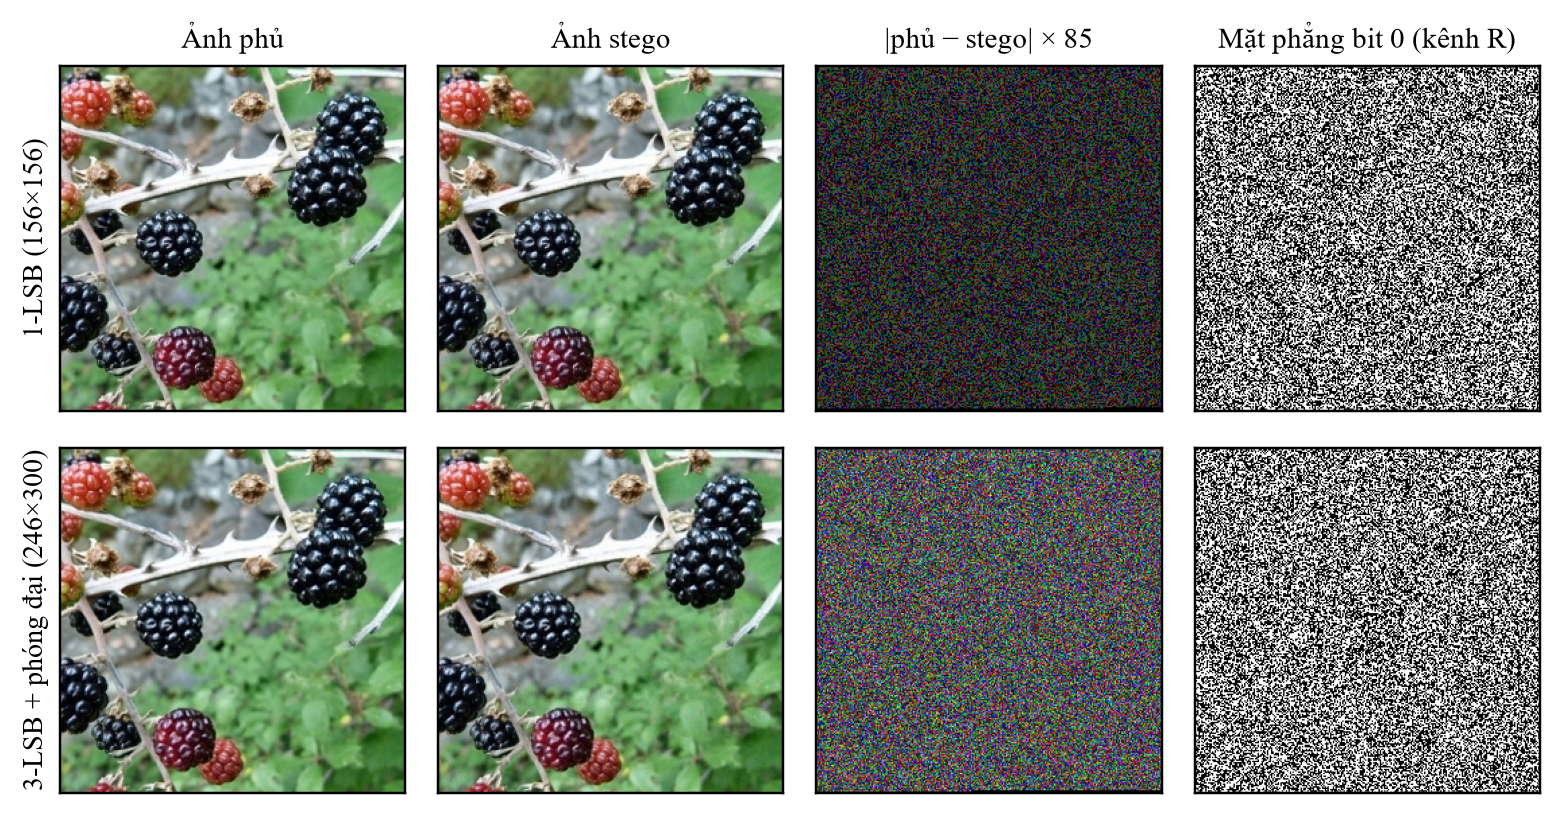
\includegraphics[width=\linewidth]{embedding_distortion}
\caption{Độ méo do nhúng: ảnh phủ, ảnh stego, sai khác tuyệt đối đã khuếch đại và mặt phẳng bit
thấp nhất (kênh R) ở hai mức tải tin}
\label{fig:distortion}
\end{figure}

\subsection{Chất lượng thị giác trên 8000 ảnh}

Ở kịch bản B, bản mã \num{24336}--\num{24352} byte cùng 128 bit header chiếm
$(128 + 8\cdot\num{24336}) / (3\cdot256^2) = 99.09\%$ số giá trị kênh. Theo \pt{eq:lsb-mse}, giá trị
kỳ vọng của MSE là $0.5\times0.9909 = 0.4954$, tương ứng PSNR $= \SI{51.18}{dB}$. Kết quả thực nghiệm
(\bang{tab:visual}, \hinh{fig:visual}) khớp gần như tuyệt đối với giá trị lý thuyết này. Toàn bộ
\num{24000} lượt chạy đều khôi phục ảnh bí mật chính xác và đều dùng 1-LSB.

\begin{table}[H]
\centering
\caption{Chất lượng thị giác trung bình trên 8000 ảnh (độ lệch chuẩn trong ngoặc)}
\label{tab:visual}
\small
\begin{tabular}{@{}llll@{}}
\toprule
\thead{Thuật toán} & \thead{MSE} & \thead{PSNR (dB)} & \thead{SSIM}\\
\midrule
3DES -- bài báo   & 0.499975 & 51.15389 & 0.998495\\
3DES -- tái hiện  & 0.495602 (0.0011) & 51.17948 (0.0099) & 0.996861 (0.0019)\\
AES -- bài báo    & 0.500006 & 51.15373 & 0.998494\\
AES -- tái hiện   & 0.495773 (0.0011) & 51.17798 (0.0098) & 0.996860 (0.0019)\\
Chaotic -- bài báo & 0.499321 & 51.14436 & 0.998099\\
Chaotic -- tái hiện & 0.495439 (0.0011) & 51.18092 (0.0097) & 0.996860 (0.0019)\\
\midrule
Lý thuyết (tải 99.09\%) & 0.4954 & 51.18 & --\\
\bottomrule
\end{tabular}
\end{table}

\begin{figure}[H]
\centering
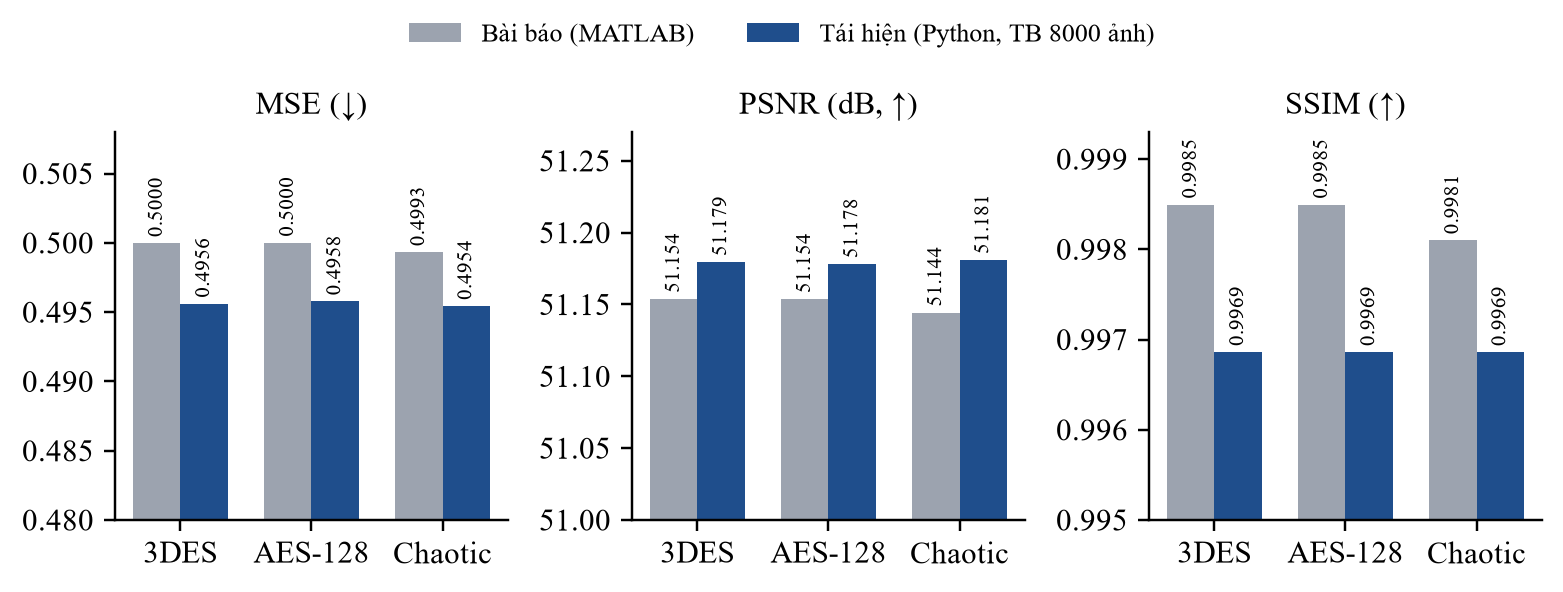
\includegraphics[width=\linewidth]{visual_paper_vs_ours}
\caption{So sánh MSE, PSNR, SSIM trung bình giữa bài báo và kết quả tái hiện}
\label{fig:visual}
\end{figure}

\begin{figure}[H]
\centering
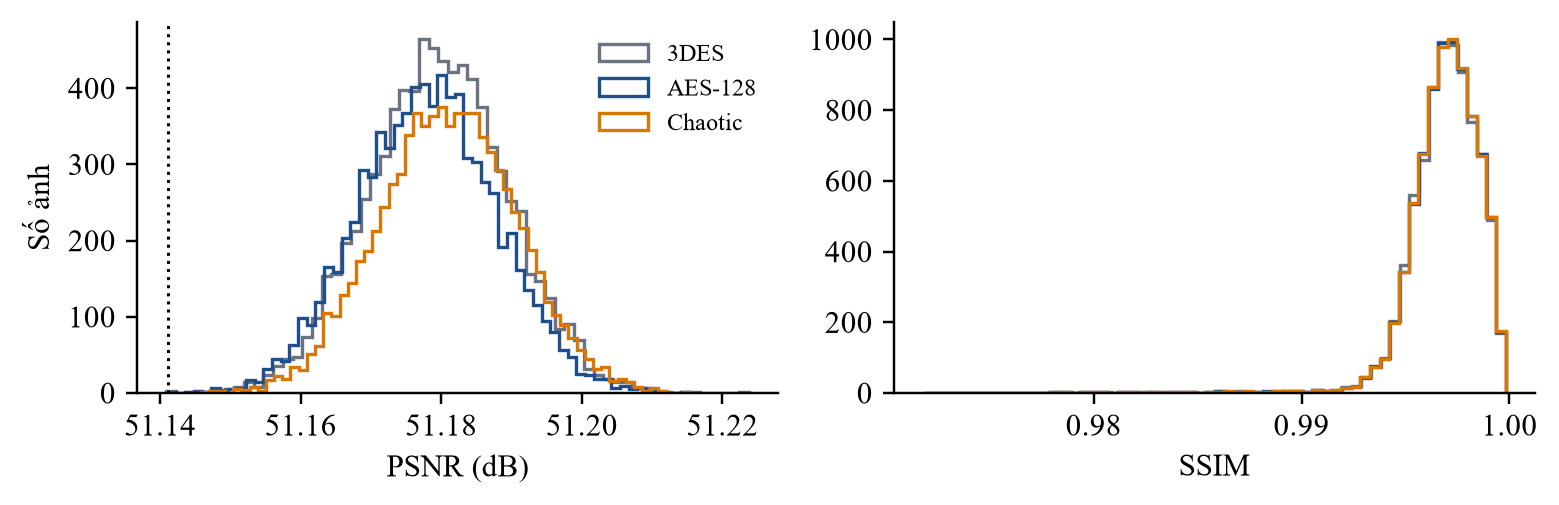
\includegraphics[width=\linewidth]{psnr_ssim_distribution}
\caption{Phân bố PSNR và SSIM trên 8000 ảnh (đường chấm: PSNR lý thuyết khi lấp đầy 100\% 1-LSB)}
\label{fig:psnr-dist}
\end{figure}

Nhận xét:
\begin{itemize}
  \item MSE và PSNR lệch bài báo dưới $1\%$ (PSNR lệch khoảng \SI{0.03}{dB}). Chênh lệch nhỏ này
        hoàn toàn do tỷ lệ lấp đầy: bài báo có MSE $\approx 0.5000$, tức đã lấp gần $100\%$ dung
        lượng 1-LSB, trong khi ảnh $156\times156$ lấp $99.09\%$.
  \item PSNR dao động rất hẹp (\SIrange{51.14}{51.22}{dB}) và gần như không phụ thuộc nội dung ảnh
        phủ hay thuật toán mã hóa, đúng như dự đoán từ \pt{eq:lsb-mse}: khi bit nhúng là ngẫu
        nhiên, độ méo chỉ phụ thuộc số bit nhúng.
  \item SSIM trung bình thấp hơn bài báo khoảng $0.0016$. Trên ảnh phủ đầu tiên (\code{berry}),
        SSIM đạt $0.99855$, gần như trùng giá trị $0.998495$ của bài báo; nhưng trên toàn bộ dữ liệu,
        các ảnh có vùng nền phẳng lớn (bầu trời, phông mờ) có SSIM thấp tới $0.972$ và kéo trung bình
        xuống. Bài báo không công bố cách tính SSIM cho ảnh màu nên không thể xác định chính xác
        nguyên nhân chênh lệch này.
\end{itemize}

\subsection{Độ an toàn thống kê của bản mã}
\label{sec:ketqua-antoan}

\bang{tab:enc-metrics} và \hinh{fig:dual} trình bày hai nhóm độ đo an toàn theo quyết định BM-08.
Một điểm quan trọng: vì khóa cố định và ảnh bí mật không đổi, bản mã của mỗi thuật toán \emph{giống
hệt nhau} trên cả 8000 lượt. Do đó các độ đo nhóm \code{*\_enc} thực chất là giá trị của một bản mã
duy nhất. Khác biệt NPCR giữa các thuật toán (ví dụ $99.59\%$ so với $99.64\%$ trong bài báo) chỉ là
dao động thống kê của một mẫu, không phản ánh thuật toán nào ``tốt hơn''.

\begin{table}[H]
\centering
\caption{Hai nhóm độ đo an toàn trung bình trên 8000 ảnh (ảnh bí mật $156\times156$)}
\label{tab:enc-metrics}
\small
\begin{tabular}{@{}lrrrr@{}}
\toprule
\thead{Độ đo} & \thead{3DES} & \thead{AES-128} & \thead{Chaotic} & \thead{Bài báo (AES)}\\
\midrule
\multicolumn{5}{@{}l}{\textit{Nhóm bản mã (ảnh bí mật -- bản mã)}}\\
NPCR\textsubscript{enc} (\%)    & 99.6548 & 99.5768 & 99.5562 & 99.6192\\
UACI\textsubscript{enc} (\%)    & 30.3253 & 30.3483 & 30.5124 & 30.8176\\
Tương quan\textsubscript{enc}   & 0.00617 & $-0.00145$ & $-0.01336$ & $-0.00407$\\
Entropy bản mã (bit)            & 7.99285 & 7.99189 & 7.99318 & --\\
\midrule
\multicolumn{5}{@{}l}{\textit{Nhóm ảnh stego (ảnh phủ -- ảnh stego)}}\\
NPCR\textsubscript{stego} (\%)  & 49.560 & 49.577 & 49.544 & --\\
UACI\textsubscript{stego} (\%)  & 0.1944 & 0.1944 & 0.1943 & --\\
Tương quan\textsubscript{stego} & 0.99989 & 0.99989 & 0.99989 & --\\
Entropy ảnh stego (bit)         & 7.46633 & 7.46633 & 7.46634 & 7.04776\\
\bottomrule
\end{tabular}
\end{table}

\begin{figure}[H]
\centering
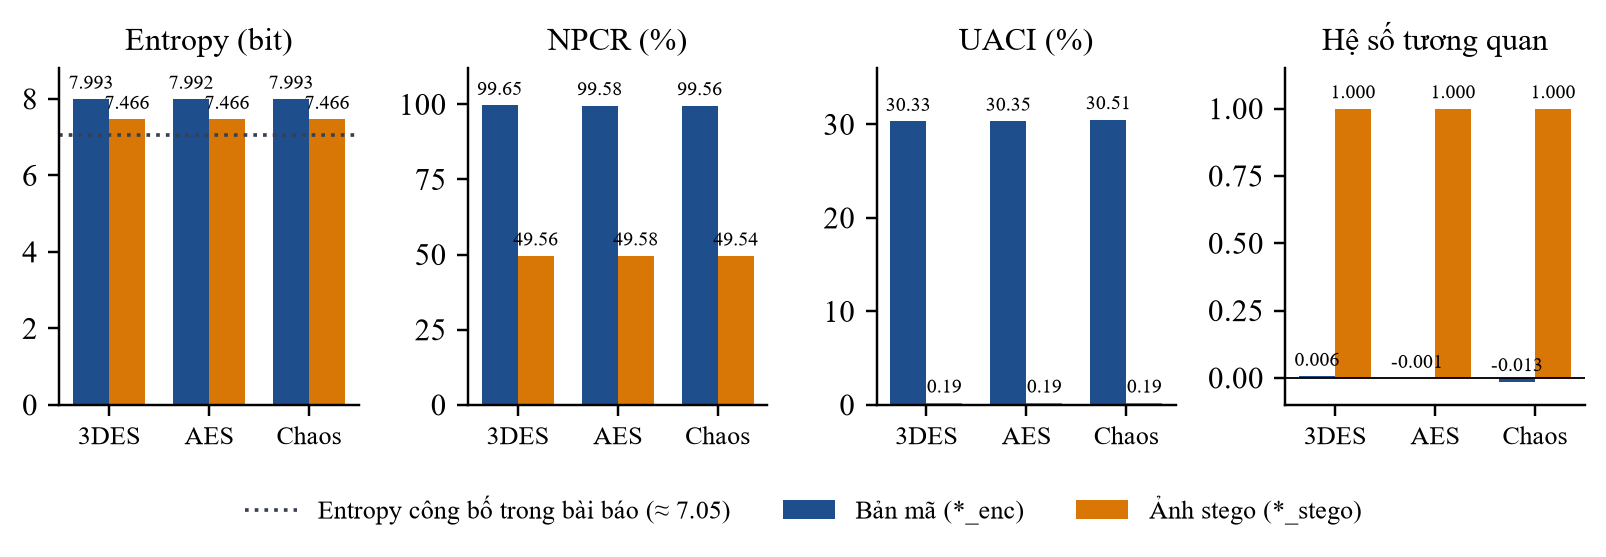
\includegraphics[width=\linewidth]{dual_metrics}
\caption{Hai nhóm độ đo: bản mã (\code{*\_enc}) và ảnh stego (\code{*\_stego})}
\label{fig:dual}
\end{figure}

Từ kết quả trên có thể giải thích đầy đủ các con số an toàn trong Bảng~2 của bài báo:
\begin{itemize}
  \item \textbf{NPCR} của cả ba thuật toán xấp xỉ giá trị lý thuyết $255/256 = 99.609\%$ của một
        bản mã ngẫu nhiên đều.
  \item \textbf{UACI} $\approx 30.3$--$30.5\%$, thấp hơn ngưỡng $33.46\%$ mà bài báo nêu. Đây
        \emph{không} phải dấu hiệu bản mã yếu. Khi so một ảnh bí mật cố định với một bản mã ngẫu
        nhiên đều $U$, giá trị kỳ vọng của UACI bằng
        $\frac{1}{mn}\sum_{i,j}\mathbb{E}\,|I(i,j) - U| / 255$ và phụ thuộc phân bố mức xám của
        ảnh bí mật. Tính trực tiếp trên ảnh ``coins'' $156\times156$ (độ sáng trung bình 96.9) cho
        giá trị kỳ vọng $30.41\%$, khớp với thực nghiệm. Ngưỡng $33.46\%$ chỉ đúng khi so hai ảnh
        ngẫu nhiên đều với nhau.
  \item \textbf{Entropy}: bản mã của cả ba thuật toán có entropy $\approx 7.992$--$7.993$ bit, sát
        cực đại 8. Giá trị $\approx 7.05$ trong bài báo nằm trong khoảng entropy của ảnh stego (ảnh
        màu tự nhiên, ở đây trung bình $7.47$), chứng tỏ bài báo đo entropy trên ảnh stego chứ
        không phải trên bản mã. Entropy của ảnh stego gần như bằng entropy của ảnh phủ và hầu như
        không phụ thuộc thuật toán mã hóa. Vì vậy kết luận của bài báo rằng Chaotic ``có entropy
        thấp hơn, cần nghiên cứu thêm về tính ngẫu nhiên'' không có cơ sở.
  \item \textbf{Tương quan} giữa ảnh bí mật và bản mã xấp xỉ 0 ở cả ba thuật toán, trong khi tương
        quan giữa ảnh phủ và ảnh stego là $0.9999$, phản ánh đúng vai trò của hai lớp: lớp mã hóa
        phá vỡ mọi liên hệ với bản rõ, lớp giấu tin giữ ảnh mang tin gần như không đổi.
\end{itemize}

Để đánh giá kỹ hơn tính ngẫu nhiên, em tính thêm tương quan giữa các điểm ảnh kề nhau và kiểm định
$\chi^2$ tính đều của histogram ($\chi^2 = \sum_i (o_i - e_i)^2/e_i$ với 255 bậc tự do, giá trị
tới hạn ở mức ý nghĩa $5\%$ là $293.25$). Kết quả ở \bang{tab:adjacent} và \hinh{fig:scatter} cho
thấy ảnh bí mật có tương quan điểm ảnh kề rất cao (0.89--0.94), còn bản mã của cả ba thuật toán có
tương quan xấp xỉ 0 và đều vượt qua kiểm định tính đều.

\begin{table}[H]
\centering
\caption{Tương quan điểm ảnh kề, entropy và kiểm định $\chi^2$ tính đều ($156\times156$)}
\label{tab:adjacent}
\small
\begin{tabular}{@{}lrrrrrc@{}}
\toprule
\thead{Ảnh} & \thead{Ngang} & \thead{Dọc} & \thead{Chéo} & \thead{Entropy} & \thead{$\chi^2$} & \thead{Đều?}\\
\midrule
Ảnh bí mật       & 0.92566 & 0.94084 & 0.88696 & 7.4252 & \num{15143.5} & \no\\
Bản mã 3DES      & $-0.00255$ & 0.00860 & 0.00398 & 7.9928 & 241.2 & \ok\\
Bản mã AES-128   & $-0.00565$ & $-0.00265$ & 0.01160 & 7.9919 & 272.3 & \ok\\
Bản mã Chaotic   & $-0.00211$ & 0.00702 & 0.00050 & 7.9932 & 231.9 & \ok\\
\bottomrule
\end{tabular}
\end{table}

\begin{figure}[H]
\centering
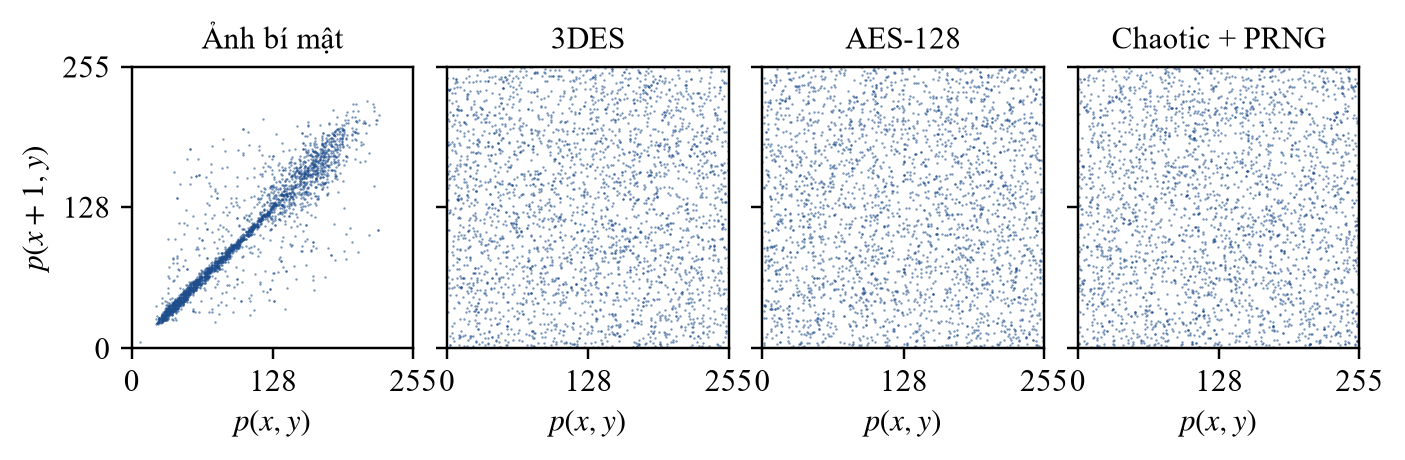
\includegraphics[width=\linewidth]{adjacent_scatter}
\caption{Phân bố cặp điểm ảnh kề theo chiều ngang (3000 cặp ngẫu nhiên)}
\label{fig:scatter}
\end{figure}

\subsection{Hiệu năng tốc độ mã hóa}

\bang{tab:enctime} và \hinh{fig:enctime} so sánh thời gian mã hóa với bài báo.

\begin{table}[H]
\centering
\caption{Thời gian mã hóa ($\mu$s) -- kịch bản B: 8000 lượt mỗi thuật toán}
\label{tab:enctime}
\small
\begin{tabular}{@{}lrrrrr@{}}
\toprule
\thead{Thuật toán} & \thead{Bài báo} & \thead{Trung bình} & \thead{Trung vị} & \thead{P95} & \thead{$246\times300$}\\
\midrule
3DES-192 CBC          & \num{3552} & \num{1303.1} & \num{1199.6} & \num{1602.2} & \num{3587.7}\\
AES-128 CBC           & 601        & 111.1        & 100.4        & 149.3        & 285.1\\
Chaotic + PRNG        & 36.2       & 31.3         & 26.0         & 51.3         & 834.5\textsuperscript{*}\\
\bottomrule
\multicolumn{6}{@{}l}{\footnotesize \textsuperscript{*} Không cache mặt nạ: thời gian gồm cả sinh \num{73800} giá trị Logistic và \num{73800} byte PRNG.}
\end{tabular}
\end{table}

\begin{figure}[H]
\centering
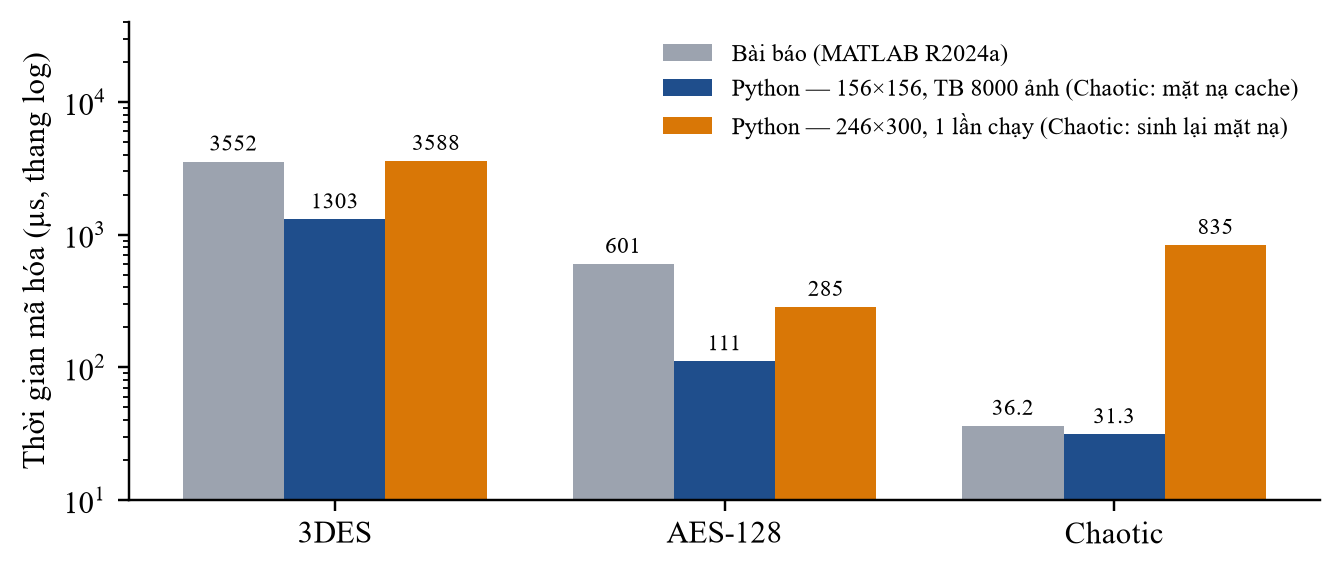
\includegraphics[width=0.9\linewidth]{enctime_compare}
\caption{Thời gian mã hóa: bài báo và kết quả tái hiện (thang logarit)}
\label{fig:enctime}
\end{figure}

\begin{figure}[H]
\centering
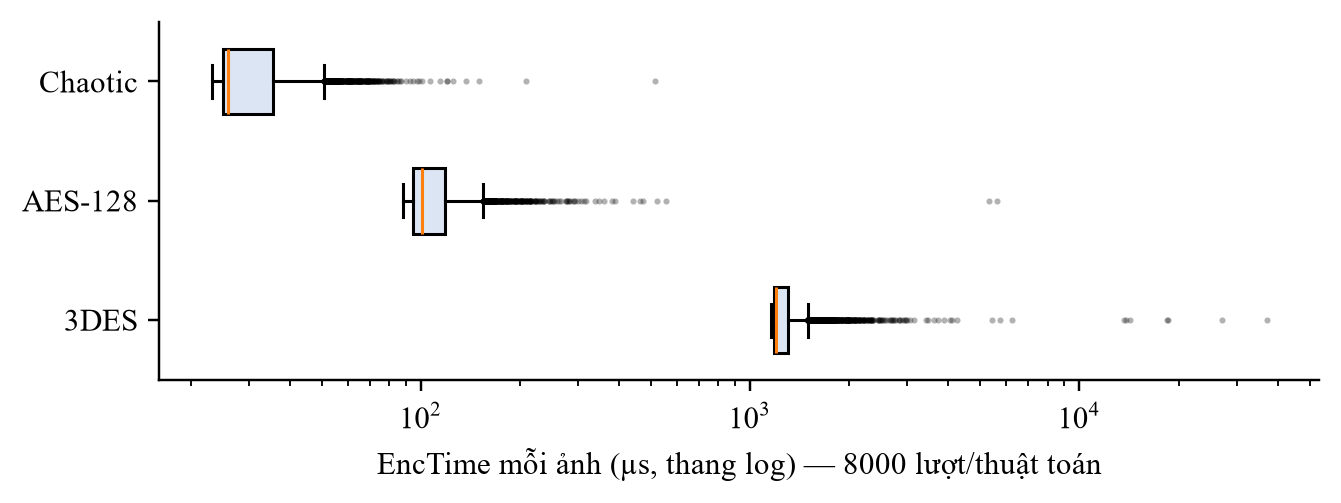
\includegraphics[width=0.9\linewidth]{enctime_distribution}
\caption{Phân bố thời gian mã hóa trên 8000 lượt chạy của mỗi thuật toán}
\label{fig:enctime-dist}
\end{figure}

Nhận xét:
\begin{itemize}
  \item Thứ tự tốc độ \textbf{Chaotic $<$ AES $<$ 3DES} của bài báo được tái hiện đúng. Với ảnh
        $156\times156$, Chaotic nhanh hơn 3DES khoảng $41.6$ lần và nhanh hơn AES khoảng $3.5$ lần;
        AES nhanh hơn 3DES khoảng $11.7$ lần.
  \item Thời gian 3DES trên ảnh $246\times300$ (\SI{3588}{\micro s}) gần như trùng giá trị
        \SI{3552}{\micro s} của bài báo. Điều này củng cố nhận định ở BM-01 rằng bài báo đo EncTime
        trên ảnh ``coins'' kích thước đầy đủ.
  \item AES trong bản tái hiện nhanh hơn bài báo khoảng $5.4$ lần nhờ PyCryptodome dùng tập lệnh
        phần cứng AES-NI. 3DES không có hỗ trợ phần cứng tương tự nên chậm hơn hẳn, vì phải chạy 48
        vòng Feistel trên khối 64 bit.
  \item Con số \SI{36.2}{\micro s} của Chaotic trong bài báo chỉ đạt được khi \emph{mặt nạ được tính
        sẵn} và chỉ đo phép XOR (chế độ cache: \SI{31.3}{\micro s}). Nếu tính cả chi phí sinh mặt nạ,
        Chaotic trên ảnh $246\times300$ mất \SI{834.5}{\micro s}, chậm hơn AES. Như vậy lợi thế tốc
        độ ``hai bậc độ lớn'' mà bài báo nêu phụ thuộc mạnh vào cách đo.
  \item Phân bố thời gian có đuôi dài (\hinh{fig:enctime-dist}) do ảnh hưởng của bộ lập lịch hệ điều
        hành và bộ nhớ đệm CPU; trung vị là đại lượng ổn định hơn trung bình khi so sánh.
\end{itemize}

\subsection{Phân tích theo lớp ảnh phủ}

Bài báo chỉ công bố giá trị trung bình gộp. Khi tách theo 5 lớp của Linnaeus 5
(\hinh{fig:class}), PSNR gần như không đổi nhưng SSIM và entropy ảnh stego khác nhau rõ rệt. Các
lớp nhiều kết cấu chi tiết như \code{dog} (SSIM $0.99721$, entropy $7.54$) và \code{berry}
($0.99709$; $7.51$) che giấu biến đổi LSB tốt hơn các lớp có nền phẳng như \code{flower}
($0.99653$) và \code{bird} ($0.99664$; entropy $7.37$). Nguyên nhân là SSIM nhạy với nhiễu $\pm1$
trên vùng phẳng hơn trên vùng nhiều chi tiết, gọi là hiệu ứng che lấp thị giác (\tn{visual
masking}). Kết quả trên tập \code{train} và \code{test} gần như trùng nhau (PSNR chênh dưới
\SI{0.001}{dB}, SSIM chênh dưới $0.0001$), cho thấy cỡ mẫu 8000 ảnh đủ để các giá trị trung bình
hội tụ.

\begin{figure}[H]
\centering
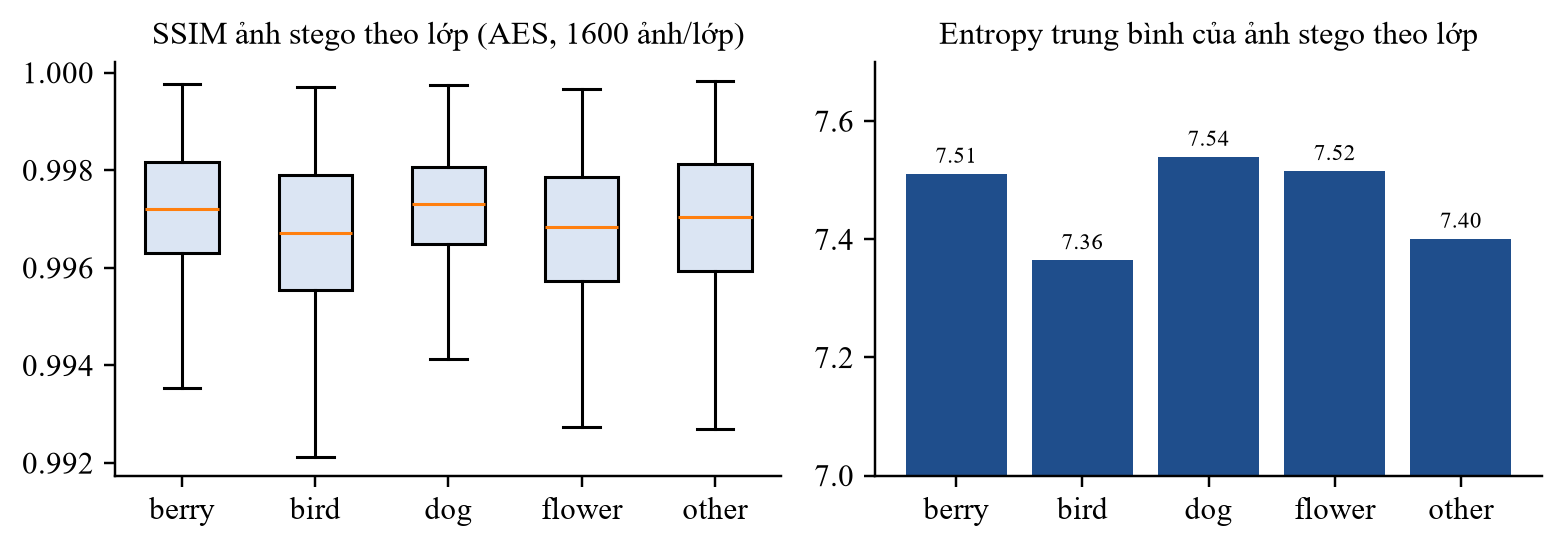
\includegraphics[width=\linewidth]{class_analysis}
\caption{SSIM và entropy ảnh stego theo 5 lớp ảnh phủ của Linnaeus 5}
\label{fig:class}
\end{figure}

\subsection{Đối chiếu tổng hợp với Bảng 2 của bài báo}

\bang{tab:compare-all} đặt cạnh nhau toàn bộ số liệu Bảng~2 của bài báo và kết quả tái hiện. Với
entropy, bản tái hiện đối chiếu cả hai cách đo.

\begin{table}[H]
\centering
\caption{Đối chiếu Bảng~2 của bài báo (BB) với kết quả tái hiện (TH) trên 8000 ảnh}
\label{tab:compare-all}
\footnotesize
\setlength{\tabcolsep}{4pt}
\begin{tabular}{@{}lrrrrrrl@{}}
\toprule
& \multicolumn{2}{c}{\thead{3DES}} & \multicolumn{2}{c}{\thead{AES-128}} & \multicolumn{2}{c}{\thead{Chaotic}} & \\
\cmidrule(lr){2-3}\cmidrule(lr){4-5}\cmidrule(lr){6-7}
\thead{Độ đo} & \thead{BB} & \thead{TH} & \thead{BB} & \thead{TH} & \thead{BB} & \thead{TH} & \thead{Mức khớp}\\
\midrule
MSE          & 0.49998 & 0.49560 & 0.50001 & 0.49577 & 0.49932 & 0.49544 & Rất sát\\
PSNR (dB)    & 51.1539 & 51.1795 & 51.1537 & 51.1780 & 51.1444 & 51.1809 & Rất sát\\
SSIM         & 0.99850 & 0.99686 & 0.99849 & 0.99686 & 0.99810 & 0.99686 & Sát\\
EncTime ($\mu$s) & 3552 & 1303 & 601 & 111 & 36.2 & 31.3 & Đúng thứ tự\\
NPCR (\%)    & 99.592 & 99.655 & 99.619 & 99.577 & 99.640 & 99.556 & Rất sát\\
UACI (\%)    & 30.808 & 30.325 & 30.818 & 30.348 & 30.961 & 30.512 & Sát, đúng thứ tự\\
Tương quan   & 0.0003 & 0.0062 & $-0.0041$ & $-0.0014$ & $-0.0098$ & $-0.0134$ & $\approx 0$\\
Entropy stego & 7.048 & 7.466 & 7.048 & 7.466 & 6.953 & 7.466 & Cùng đối tượng\\
Entropy bản mã & -- & 7.993 & -- & 7.992 & -- & 7.993 & Bài báo không đo\\
\bottomrule
\end{tabular}
\end{table}

Có thể kết luận bản tái hiện khớp với bài báo ở các điểm chính: MSE, PSNR, NPCR khớp gần như tuyệt
đối; UACI và SSIM khớp ở mức sát với chênh lệch đã được giải thích; thứ tự tốc độ được giữ nguyên.
Riêng entropy ảnh stego của bản tái hiện ($7.47$) cao hơn bài báo ($7.05$). Đây là đại lượng phụ
thuộc hoàn toàn vào ảnh phủ chứ không vào thuật toán, nên khác biệt có thể đến từ cách bài báo tính
entropy cho ảnh màu (ví dụ chuyển sang ảnh xám trước khi tính).

% =====================================================================
\section{Phân tích an toàn mở rộng}
\label{sec:antoan-morong}
% =====================================================================

Các độ đo trong bài báo chủ yếu mô tả \emph{tính thống kê} của bản mã và ảnh stego. Một hệ mật mã
chỉ có thể coi là an toàn khi chịu được các mô hình tấn công cụ thể. Phần này đánh giá thêm năm khía
cạnh mà bài báo chưa đề cập, dùng chính mã nguồn đã cài đặt và ảnh bí mật $156\times156$.

\subsection{Độ nhạy khóa}

Một hệ mật tốt phải cho bản mã khác hoàn toàn khi khóa thay đổi dù rất nhỏ, và giải mã bằng khóa
gần đúng không được tiết lộ thông tin. \bang{tab:keysens} cho thấy cả ba thuật toán đều đạt yêu cầu
này: đảo một bit khóa 3DES/AES, hay thay đổi $x_0$ hoặc $r$ chỉ $10^{-10}$, đều làm khoảng $99.3$--$99.6\%$
điểm ảnh bản mã thay đổi, UACI xấp xỉ $33.4\%$ (giá trị của hai ảnh ngẫu nhiên độc lập), và ảnh giải
mã bằng khóa sai chỉ còn là nhiễu (PSNR $\approx \SI{8.7}{dB}$). Với Chaotic, NPCR thấp hơn đôi chút
($99.3\%$) vì hai quỹ đạo Logistic chỉ tách nhau sau khoảng 30 bước lặp (\hinh{fig:logistic}b), nên
vài chục byte đầu của hai bản mã trùng nhau.

\begin{table}[H]
\centering
\caption{Độ nhạy khóa: so sánh bản mã của khóa đúng và khóa bị thay đổi rất nhỏ}
\label{tab:keysens}
\small
\begin{tabularx}{\linewidth}{@{}lLrrr@{}}
\toprule
\thead{Thuật toán} & \thead{Thay đổi khóa} & \thead{NPCR (\%)} & \thead{UACI (\%)} & \thead{PSNR giải mã sai}\\
\midrule
3DES    & Đảo 1 bit của $K_1$ (bit 1, byte 0) & 99.626 & 33.385 & \SI{8.61}{dB}\\
AES-128 & Đảo 1 bit của khóa (bit 0, byte 0)  & 99.552 & 33.466 & \SI{8.63}{dB}\\
Chaotic & $x_0 \to x_0 + 10^{-10}$            & 99.310 & 32.708 & \SI{8.72}{dB}\\
Chaotic & $r \to r + 10^{-10}$                & 99.240 & 32.771 & \SI{8.71}{dB}\\
Chaotic & \code{ecc\_seed}: $42 \to 43$       & 99.643 & 33.390 & \SI{8.72}{dB}\\
\bottomrule
\end{tabularx}
\end{table}

\subsection{Độ nhạy bản rõ -- phân tích vi sai đúng định nghĩa}

Trong phân tích vi sai chuẩn \cite{wu2011npcr}, kẻ tấn công mã hóa hai ảnh chỉ khác nhau \emph{một
điểm ảnh} rồi so sánh hai bản mã. Lược đồ tốt phải cho NPCR $\approx 99.6\%$ để không có quan hệ
khai thác được giữa thay đổi bản rõ và thay đổi bản mã. \bang{tab:plainsens} cho kết quả khi tăng
giá trị một điểm ảnh lên 1 ở ba vị trí khác nhau.

\begin{table}[H]
\centering
\caption{Độ nhạy bản rõ: NPCR/UACI (\%) giữa hai bản mã khi ảnh bí mật đổi đúng một điểm ảnh}
\label{tab:plainsens}
\small
\begin{tabular}{@{}lrrr@{}}
\toprule
\thead{Vị trí điểm ảnh thay đổi} & \thead{3DES} & \thead{AES-128} & \thead{Chaotic}\\
\midrule
Đầu ảnh $(0, 0)$        & 99.626 / 33.520 & 99.667 / 33.600 & 0.0041 / 0.00002\\
Giữa ảnh $(78, 78)$     & 49.511 / 16.594 & 49.466 / 16.483 & 0.0041 / 0.00005\\
Cuối ảnh $(155, 155)$   & 0.0329 / 0.0151 & 0.0657 / 0.0272 & 0.0041 / 0.00008\\
\bottomrule
\end{tabular}
\end{table}

Kết quả phản ánh đúng cấu trúc của từng thuật toán:
\begin{itemize}
  \item Với CBC, thay đổi ở khối $P_i$ lan sang mọi khối \emph{phía sau} theo \pt{eq:cbc}. Thay đổi
        điểm ảnh đầu làm toàn bộ bản mã thay đổi, ở giữa ảnh thì khoảng một nửa, còn ở điểm ảnh cuối
        thì chỉ đúng một khối thay đổi (8 byte $= 0.033\%$ với 3DES, 16 byte $= 0.066\%$ với AES).
  \item Với Chaotic + PRNG, dòng khóa không phụ thuộc bản rõ nên thay đổi một điểm ảnh chỉ làm
        \emph{đúng một byte} bản mã thay đổi ($1/\num{24336} = 0.0041\%$). Lược đồ hoàn toàn không có
        tính khuếch tán.
\end{itemize}
Như vậy, NPCR $\approx 99.6\%$ trong bài báo (đo giữa ảnh bí mật và bản mã) \emph{không} chứng minh
được khả năng chống tấn công vi sai. Khi đo đúng định nghĩa, Chaotic thất bại hoàn toàn, còn 3DES và
AES ở chế độ CBC với IV cố định chỉ đạt yêu cầu khi thay đổi nằm ở đầu ảnh.

\subsection{Tấn công biết bản rõ lên lớp Chaotic + PRNG}

Mặt nạ của lớp Chaotic được sinh từ các tham số cố định $(x_0, r, \mathit{seed})$, không phụ thuộc
bản rõ và không có số dùng một lần (\tn{nonce}). Vì vậy mọi ảnh đều được XOR với \emph{cùng một dòng
khóa} và lược đồ rơi vào đúng trường hợp dùng lại dòng khóa ở \pt{eq:twotime}. Em mô phỏng một kẻ tấn
công biết một cặp (ảnh bí mật $A$, bản mã $C_A$), ví dụ một ảnh đã từng bị lộ, và thu được bản mã
$C_B$ của một ảnh khác $B$ (ảnh ``camera''). Kết quả ở \hinh{fig:kpa}:
\begin{itemize}
  \item Chỉ cần XOR hai bản mã, $C_A \xor C_B = A \xor B$ đã lộ rõ đường nét chồng lên nhau của cả
        hai ảnh (hệ số tương quan với $A \xor B$ bằng $1.0$);
  \item Dòng khóa khôi phục được bằng $A \xor C_A$, từ đó giải mã được $B = C_B \xor (A \xor C_A)$
        \textbf{chính xác 100\%} mà không cần biết $x_0$, $r$ hay seed;
  \item Cùng phép tấn công đó với AES-CBC chỉ cho ra nhiễu (PSNR \SI{7.84}{dB}, tương quan $0.005$),
        vì AES là hoán vị giả ngẫu nhiên chứ không phải phép XOR với dòng khóa cố định.
\end{itemize}

\begin{figure}[H]
\centering
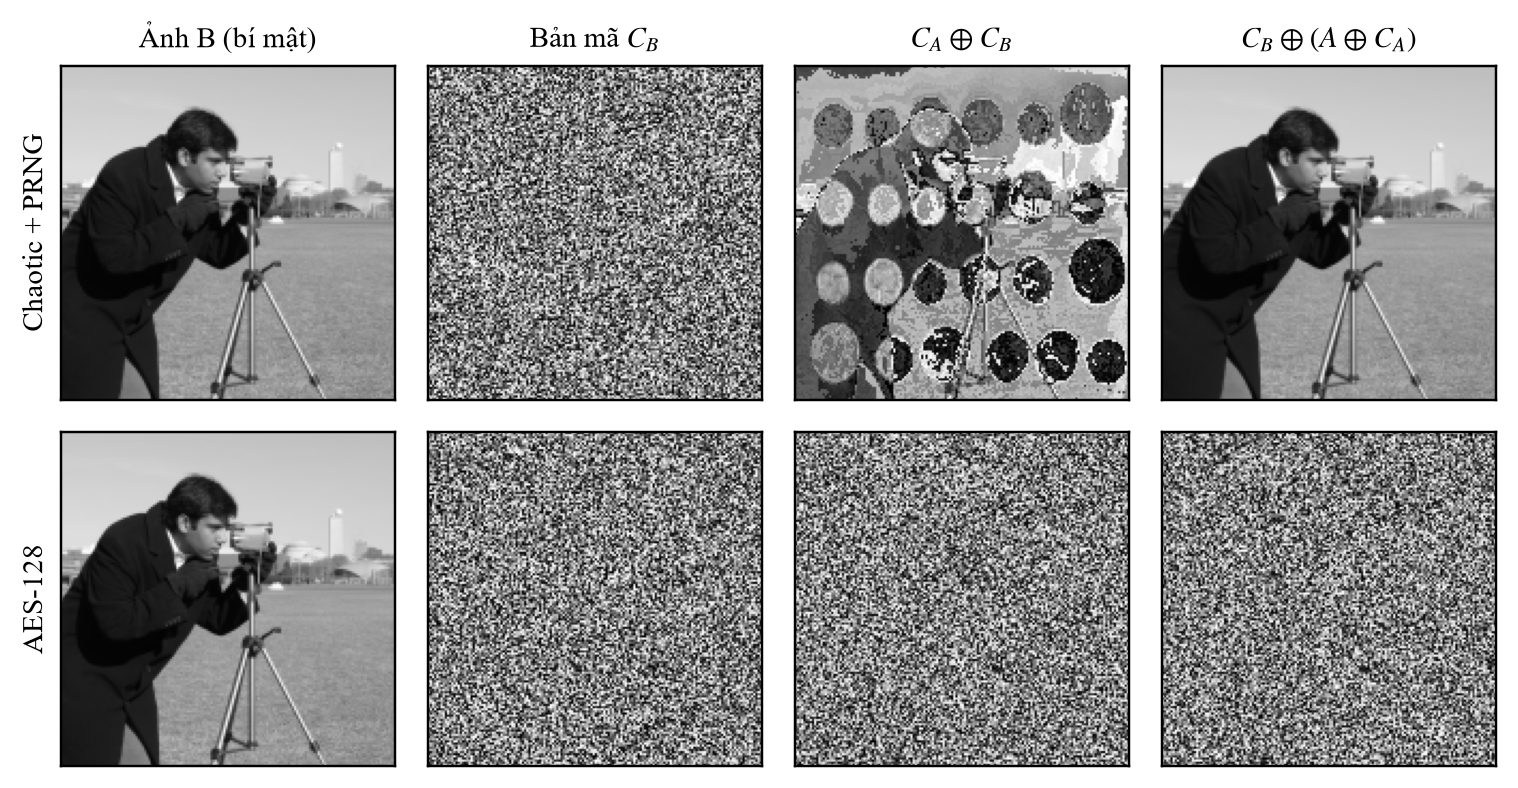
\includegraphics[width=0.95\linewidth]{kpa_attack}
\caption{Tấn công biết bản rõ: lớp Chaotic + PRNG bị phá hoàn toàn, AES-CBC không bị ảnh hưởng}
\label{fig:kpa}
\end{figure}

Ngoài ra, bài báo công bố công khai $x_0 = 0.785398$, $r = 3.999$, và mặt nạ ``ECC'' chỉ phụ thuộc
một seed số nguyên. Không gian khóa thực tế vì thế rất nhỏ so với 112 bit của 3DES hay 128 bit của
AES, vi phạm cả nguyên lý Kerckhoffs lẫn các yêu cầu cơ bản cho hệ mật hỗn loạn mà Alvarez và Li đã
nêu \cite{alvarez2006}. Kết luận rằng phương pháp hỗn loạn ``an toàn và nhanh hơn'' của bài báo vì
vậy cần được hiểu thận trọng: nó nhanh hơn chính vì nó chỉ là một mã dòng đơn giản dùng lại khóa.

\subsection{Khả năng chống chỉnh sửa}

Dùng phòng thí nghiệm tấn công của ứng dụng (Tab~2), em áp dụng năm kịch bản lên ảnh stego của cả ba
thuật toán. Kết quả tổng hợp ở \bang{tab:tamper} và \hinh{fig:tamper}.

\begin{table}[H]
\centering
\caption{Phản ứng của hệ thống trước các kịch bản tấn công/chỉnh sửa ảnh stego}
\label{tab:tamper}
\small
\begin{tabularx}{\linewidth}{@{}P{3.3cm}P{2.5cm}LL@{}}
\toprule
\thead{Kịch bản} & \thead{Dừng ở bước} & \thead{3DES / AES-128} & \thead{Chaotic}\\
\midrule
Không tấn công & -- & Khôi phục chính xác & Khôi phục chính xác\\
Giải mã sai khóa (seed + 1) & Giải mã & Phát hiện: lỗi gỡ đệm PKCS\#7; dữ liệu thô là nhiễu (PSNR 8.66/8.67 dB) & Không phát hiện: trả về ảnh nhiễu như kết quả hợp lệ (PSNR 8.72 dB)\\
Nén JPEG Q = 95 & Header & \multicolumn{2}{l}{Phát hiện: sai magic \code{HCST}, toàn bộ LSB bị phá hủy}\\
Đảo 1 bit trong header & Header & \multicolumn{2}{l}{Phát hiện: CRC-16 không khớp}\\
Đảo 1\% bit payload & Giải mã & Lỗi lan truyền theo khối: BER 24.1\% / 35.9\%, PSNR 11.9 / 10.0 dB; lần này lỗi đệm báo hiệu & Không phát hiện: BER đúng 1.0\%, PSNR 24.9 dB, lỗi rải rác\\
Nhiễu Gauss $\sigma = 2$ & Header & \multicolumn{2}{l}{Phát hiện: sai magic \code{HCST}}\\
\bottomrule
\end{tabularx}
\end{table}

\begin{figure}[H]
\centering
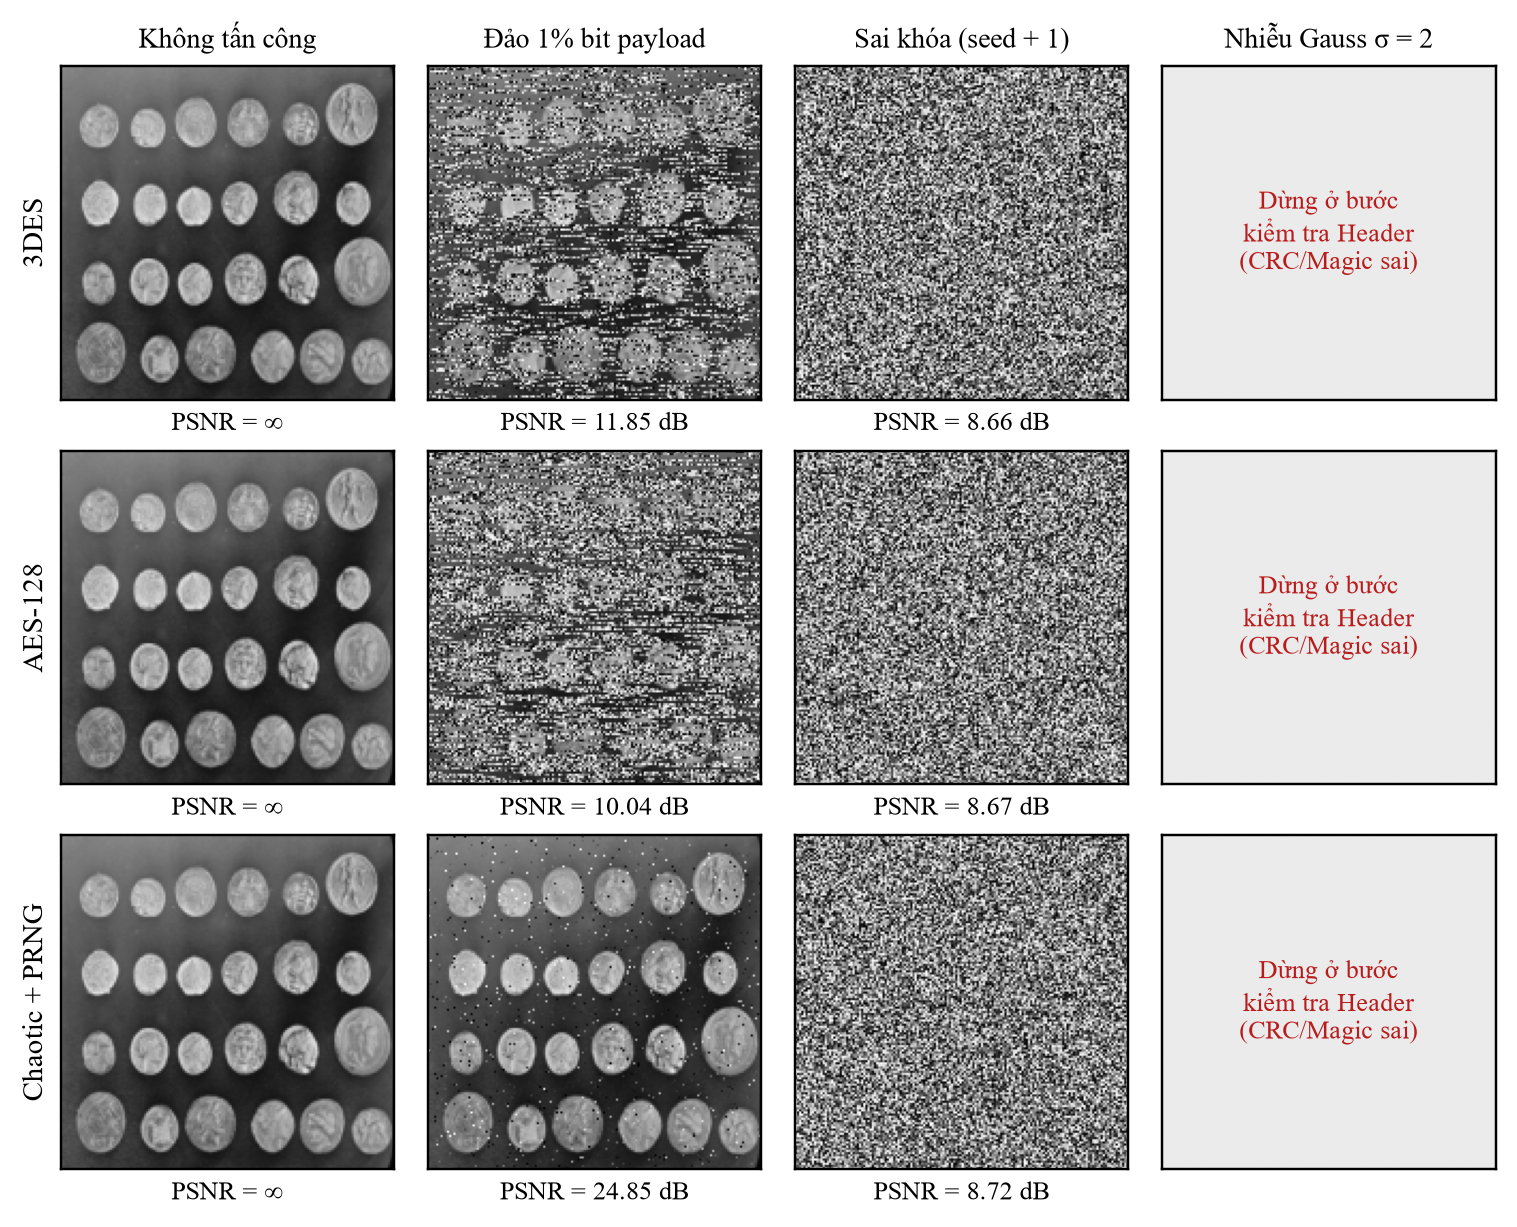
\includegraphics[width=0.92\linewidth]{tamper_grid}
\caption{Ảnh khôi phục dưới các kịch bản tấn công (cột cuối: bị chặn ngay ở bước kiểm tra header)}
\label{fig:tamper}
\end{figure}

Những nhận xét rút ra:
\begin{itemize}
  \item Giấu tin LSB thay thế là kỹ thuật \emph{mong manh} (\tn{fragile}): chỉ một lần nén JPEG chất
        lượng cao hoặc nhiễu rất nhỏ cũng phá hủy toàn bộ thông điệp. Header có magic và CRC-16 giúp
        hệ thống phát hiện ngay các trường hợp này thay vì giải mã ra dữ liệu rác, nhưng không khôi
        phục được thông điệp.
  \item CRC-16 chỉ phát hiện sai lệch ngẫu nhiên. Kẻ tấn công chủ động có thể sửa header rồi tính
        lại CRC. Phần payload hoàn toàn không được bảo vệ toàn vẹn: với 3DES/AES, việc phát hiện chỉ
        là ``tình cờ'' khi khối cuối bị hỏng làm sai đệm PKCS\#7; với Chaotic thì không có bất kỳ cơ
        chế phát hiện nào.
  \item Ở khía cạnh độ bền, Chaotic lại có ưu điểm: lỗi bit không lan truyền nên ảnh khôi phục vẫn
        nhận ra được (PSNR \SI{24.9}{dB}), trong khi CBC khuếch đại mỗi bit lỗi thành cả một khối
        hỏng.
\end{itemize}

\subsection{Khả năng bị phát hiện bởi phân tích giấu tin}

Mục tiêu cốt lõi của lớp giấu tin là không bị phát hiện. Tuy nhiên, ở chế độ 1-LSB lấp $99\%$ dung
lượng, mặt phẳng bit thấp nhất của ảnh stego bị thay hoàn toàn bằng dữ liệu ngẫu nhiên
(\hinh{fig:lsb-plane}). Trong khi đó mặt phẳng bit thấp của ảnh tự nhiên vẫn còn mang dấu vết cấu trúc
của ảnh, đặc biệt ở các vùng bão hòa hoặc phẳng.

\begin{figure}[H]
\centering
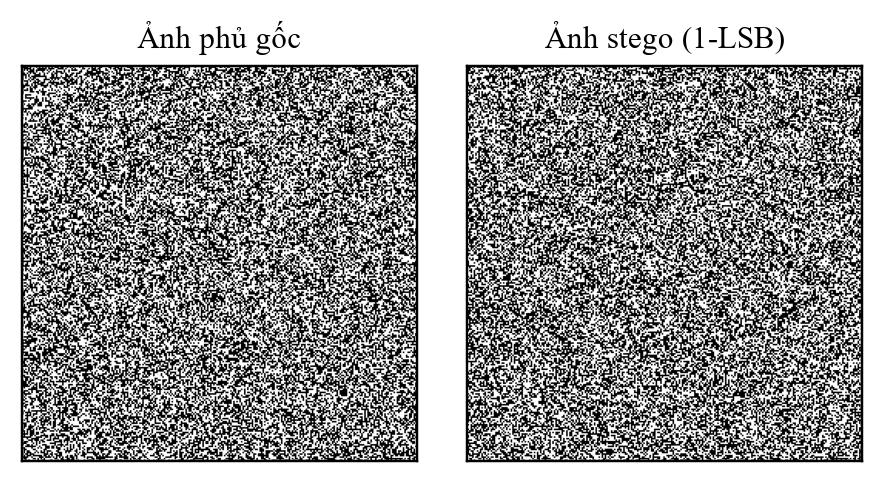
\includegraphics[width=0.62\linewidth]{lsb_plane}
\caption{Mặt phẳng bit thấp nhất (kênh R) của ảnh phủ và ảnh stego}
\label{fig:lsb-plane}
\end{figure}

Em áp dụng kiểm định $\chi^2$ trên cặp giá trị của Westfeld và Pfitzmann \cite{westfeld2000} cho cả
8000 ảnh phủ và 8000 ảnh stego tương ứng (AES, $156\times156$). Ảnh được coi là ``có giấu tin'' khi
giá trị $p > 0.95$. Kết quả (\hinh{fig:chi2}):
\begin{itemize}
  \item \textbf{99.84\%} ảnh stego bị phát hiện (trung vị $p = 0.999999$);
  \item chỉ \textbf{4.58\%} ảnh phủ gốc bị báo nhầm (trung vị $p \approx 2.4\times10^{-24}$).
\end{itemize}
Như vậy, với một phép kiểm định thống kê đơn giản công bố từ năm 1999, kẻ tấn công gần như luôn biết
ảnh nào đang mang tin. Lớp giấu tin của bài báo vì thế không đạt được mục tiêu ``vô hình'' trước một
đối thủ có kiến thức, dù đạt PSNR rất cao trước mắt người. Lý do là LSB \emph{thay thế} làm cân bằng
tần suất của các cặp giá trị $(2k, 2k+1)$, một dấu vết mà ảnh tự nhiên không có.

\begin{figure}[H]
\centering
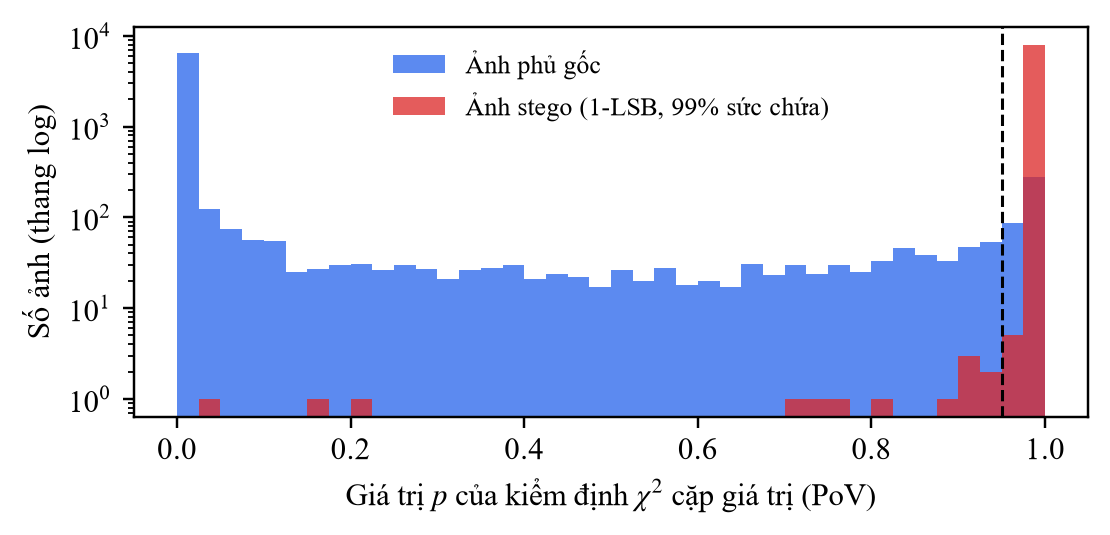
\includegraphics[width=0.82\linewidth]{chi2_steganalysis}
\caption{Phân bố giá trị $p$ của kiểm định $\chi^2$ cặp giá trị trên 8000 ảnh phủ và 8000 ảnh stego
(đường đứt: ngưỡng $p = 0.95$)}
\label{fig:chi2}
\end{figure}

\subsection{Tổng hợp đánh giá và đề xuất cải tiến}

\bang{tab:improve} tổng hợp các hạn chế đã được kiểm chứng bằng thực nghiệm và hướng khắc phục tương
ứng.

\begin{table}[H]
\centering
\caption{Các hạn chế đã kiểm chứng và đề xuất cải tiến}
\label{tab:improve}
\small
\begin{tabularx}{\linewidth}{@{}P{4.5cm}L@{}}
\toprule
\thead{Hạn chế} & \thead{Đề xuất khắc phục}\\
\midrule
Chaotic dùng lại dòng khóa; tham số công khai; không khuếch tán
  & Dẫn xuất dòng khóa từ khóa bí mật và một nonce ngẫu nhiên lưu trong header; tốt hơn là dùng mã dòng chuẩn như ChaCha20\\
IV cố định cho CBC: hai ảnh giống phần đầu cho bản mã giống phần đầu
  & Sinh IV ngẫu nhiên cho mỗi lần mã hóa và lưu vào header (IV không cần bí mật)\\
Không xác thực bản mã; CRC không chống sửa đổi có chủ đích
  & Dùng mã hóa có xác thực AES-GCM \cite{sp80038d} (hoặc ChaCha20-Poly1305) và đưa header vào dữ liệu liên kết (AAD) để mọi sửa đổi đều bị phát hiện\\
Khóa dẫn xuất từ seed công khai / SHA-256 của mật khẩu
  & Dùng hàm dẫn xuất khóa chậm có muối như Argon2 \cite{rfc9106} hoặc PBKDF2\\
3DES đã bị NIST loại bỏ, khối 64 bit dễ bị tấn công va chạm
  & Chỉ giữ 3DES để so sánh; dùng AES cho ứng dụng thực tế\\
LSB thay thế dễ bị kiểm định $\chi^2$ phát hiện
  & Dùng LSB matching ($\pm1$) \cite{mielikainen2006}, hoán vị vị trí nhúng bằng khóa, giảm tỷ lệ tải tin hoặc dùng giấu tin thích nghi \cite{holub2014}\\
Giấu tin không bền trước nén và nhiễu
  & Nếu cần độ bền: kết hợp mã sửa lỗi và nhúng trong miền biến đổi (DCT/DWT), chấp nhận giảm dung lượng\\
\bottomrule
\end{tabularx}
\end{table}
